\documentclass[pt12]{article}
%.
\usepackage[margin=1in, paperwidth=8.5in, paperheight=11in]{geometry}
\usepackage{amsfonts}
\usepackage{amsmath}
\usepackage[margin=1in]{geometry}
\usepackage{amsfonts,amsmath,amssymb}
\usepackage[none]{hyphenat}
\usepackage{fancyhdr}
\usepackage{graphicx}
\usepackage{float}
\usepackage{xcolor}
\usepackage[nottoc,notlot,notlof]{tocbibind}
\usepackage{hyperref}
%.
\pagestyle{fancy}
\fancyhead{}
\fancyfoot{}
\fancyhead[L]{\slshape \MakeUppercase{Métodos de Monte Carlo - Quasi-Random}}
\fancyhead[R]{\slshape Erik Davino Vincent}
\fancyfoot[C]{\thepage}
%.
\makeatletter
\newcommand{\rmnum}[1]{\romannumeral #1}
\newcommand{\Rmnum}[1]{\expandafter\@slowromancap\romannumeral #1@}
\makeatother


\begin{document}

\begin{titlepage}

\title{\textbf{Relatório do Exercício Programa 5:\\FBST - Hardy-Weinberg Equilibrium Law}}
\author{Erik Davino Vincent - BMAC - Turma 54 \\ NUSP: 10736584}
\date{\today}
\maketitle
\line(1,0){440}
\ \\
\ \\
\ \\
\ \\
\ \\
\ \\
\ \\
\ \\
\begin{center}


\includegraphics[scale=0.1]{ime.png}\\
\ \\
\ \\
\begin{LARGE}\tt{IME - USP} \end{LARGE}


\end{center}

\end{titlepage}

\tableofcontents

\newpage

\begin{center}\section{Introdução}\end{center}
\

\textbf{Algorítimo pode ser encontrado no arquivo EP5.py e resultados apresentados, tal como aparecem no programa estão nos arquivos Resultados(Auto).txt e Resultados(non-Auto).txt, que vieram no arquivo compactado.}\\
\ 

O seguinte relatório tem como objetivo analisar os resultados reproduzidos da Sec. 4-3 (Hardy-Weinberg Equilibrium Law) do artigo\\
\ 

C.A.B.Pereira, J.M.Stern (1999). Evidence and Credibility: Full Bayesian
Signicance Test for Precise Hypotheses. Entropy Journal, 1, 69-80.\\
\ 

para os testes de hipótese de e-valor, para cada vetor $\vec{X} = (x_1,x_2,x_3)$ presente na tabela do artigo. Para tanto, foi utilizado um passo de otimização e um passo de integração, via um algorítimo de Markov-Chain Monte Carlo.\\
\ 

\subsection{O problema}
\ 

Possuímos uma função de probabilidade $\displaystyle{Pn(\theta|x) \propto \theta_1^{x_1}\cdot\theta_2^{x_2}\cdot\theta_3^{x_3}}$, tal que $\theta = (\theta_1, \theta_2, \theta_3)$, definida no espaço $\Theta$ o qual possui as seguintes restrições:

\begin{enumerate}
\item $\theta \geq 0$
\item $\theta_1+\theta_2+\theta_3 = 1$.
\end{enumerate}

E queremos verificar para um dado vetor $(x_1,x_2,x_3)$ se a hipótese
$$\displaystyle{\theta_3 = (1 - \sqrt{\theta_1})^2}$$
é verdadeira. O espaço da hipótese, $H$, é restrito por:

\begin{enumerate}
\item $\theta \geq 0$
\item $\theta_1+\theta_2+\theta_3 = 1$
\item $\displaystyle{\theta_3 = (1 - \sqrt{\theta_1})^2}$.
\end{enumerate}

Queremos fazer o teste do e-valor para medir o quanto a nossa hipótese se aproxima do espaço paramétrico, dado um conjunto de xizes. Para tal, temos duas etapas:\\
\ 

\section{Otimização (Cálculo no espaço da hipótese)}
\ 

O passo da otimização consiste em encontrar $\theta^* = \max_{\theta \in H}Pn(\theta|x)$, o que equivale a dizer que $\theta^* = \arg\max Pn(\theta|x)$. Ou seja, $\theta^*$ é o parâmetro que maximiza a função $Pn$.\\
\ 

As restrições do espaço da hipótese nos permitem facilmente fazer a otimização, se reparametrizarmos $Pn$ para depender somente de $\theta_1$:

\begin{enumerate}
\item $\theta \geq 0 \iff \theta_1 \geq 0 \text{ e } \theta_2 \geq 0 \text{ e } \theta_3 \geq 0$
\item $\theta_1+\theta_2+\theta_3 = 1 \iff \theta_2 = 1 - \theta_1 - \theta3 \iff 1 > \theta_1 + \theta_3$
\item $\theta_3 = (1-\sqrt{\theta_1})^2 \iff \theta_2 = 1 - \theta_1 - (1-\sqrt{\theta_1})^2$
\item (1, 2 e 3) $\implies \displaystyle{Pn(\theta |x) \propto \theta_1^{x_1}\cdot(1 - \theta_1 - [1 - \sqrt{\theta1}]^2)^{x_2}\cdot([1-\sqrt{\theta_1}]^2)^{x_3}}$.
\end{enumerate}

Dada a nova parametrização de $Pn$, basta encontrar $\theta_1$ que maximiza $Pn$.\\
\ 

\subsection{Algorítimo de otimização}
\ 

Para fazer a otimização, não necessitei de qualquer biblioteca ou função já pronta. Ao invés disso, como apenas precisávamos encontrar $Pn$ máximo dentro de um intervalo conhecido e finito, $[0,1]$, o algorítimo consiste numa busca simples pelo máximo:

\begin{enumerate}
\item Dado um número $n$ de iterações:
\item Verificar dentre $n$ pontos equidistantes no intervalo $[0,1]$ qual leva ao maior $Pn$
\end{enumerate}

Supõe-se que para um número suficientemente grande de iterações (digamos 5000), podemos encontrar o $Pn$ máximo, logo $\theta^*$, com uma precisão bem alta, e pouco esforço computacional.\\
\ 

Uma alternativa possível, seria buscar o máximo por pontos aleatórios, ou até mesmo MCMC, porém, o resultado provavelmente seria igual ou pior, no mínimo mais inconsistente, pois iria variar para cada execução do algorítimo.\\

\begin{small}
$^*$Para mais informações do algorítimo, vide arquivo EP5.py
\end{small}\\
\ 

\section{Integração (cálculo no espaço paramétrico}
\ 

O passo de integração decorre de que
$$ev(h|x) = 1-\int_{\Gamma}Pn(\theta)$$
tal que $\displaystyle{\Gamma = \{ \theta \in \Theta|Pn(\theta) > Pn(\theta^*)\}}$. Ou seja, queremos integrar $Pn(\theta)$ na região delimitada pela curva de nível com altura $Pn(\theta^*)$. Para tanto utilizamos um MCMC com caminho em duas dimensões, isso é, dependente de duas variáveis, $\theta_1$ e $\theta_3$.\\
\ 

Podemos fazer o MCMC em duas variáveis apenas, devido as restrições de $\Theta$:

\begin{enumerate}
\item $\theta \geq 0 \iff \theta_1 \geq 0 \text{ e } \theta_2 \geq 0 \text{ e } \theta_3 \geq 0$
\item $\theta_1+\theta_2+\theta_3 = 1 \iff \theta_2 = 1 - \theta_1 - \theta3 \iff 1 > \theta_1 + \theta_3$
\item (1 e 2) $\implies \displaystyle{Pn(\theta|x) \propto \theta_1^{x_1}\cdot(1 - \theta_1 - \theta_3)^{x_2}\cdot\theta_3^{x_3}}$
\end{enumerate}

Dessa forma, basta fazer a amostra de pontos $X_i = (\theta_{1i},\theta_{3i})\sim Pn(\theta|x)$ a partir do MCMC e verificar para cada $Pn(X_i)$ se seu valor é maior do que $Pn(\theta^*)$.\\
\ 

\subsection{Algorítimo do MCMC e da Integração}
\ 

O algorítimo utilizado para fazer o MCMC de $Pn$ é o mesmo utilizado no Exercício Programa 4, com a simples diferença de que o caminho aleatório é feito em duas dimensões, logo, com um núcleo bidimensional. No caso, foi utilizado um núcleo $N_2(0,\Sigma)$, um núcleo Normal bi-variado com média $0$ e variância $\Sigma$, uma matriz de covariância definida como:

$$\Sigma = \begin{pmatrix}
\sigma_1^2 & 0\\
0 & \sigma_2^2
\end{pmatrix}$$

Isso é o mesmo que dizer que, dado um ponto atual da cadeia, $(\theta_{1i},\theta_{3i})$, o próximo ponto candidato será escolhido na posição aleatória $\sim Normal(\theta_{1i},\sigma_1^2)$ na direção do eixo de $\theta_1$ e na posição aleatória $\sim Normal(\theta_{3i},\sigma_2^2)$ na direção do eixo de $\theta_3$.
Dessa forma, cada ponto $(\theta_{1i},\theta_{3i})$ é escolhido independentemente por uma função $Normal$.\\
\ 

Sobre a integração: basta verificar a proporção de pontos do MCMC que satisfazem $Pn(\theta)>Pn(\theta^*)$. Para verificar o e-valor, subtrair esse valor de $1$.
\subsubsection{Escolha do $\alpha$}
\ 

O resto do algorítimo é exatamente igual, basicamente o algorítimo de Metropolis adaptado para duas variáveis. Como o núcleo é simétrico, vale que $\displaystyle{\alpha = \min\left(1,\frac{Pn(\theta_{prox})}{Pn(\theta_{atual})}\right)}$. O $\alpha$ utilizado foi nesse caso o de Metropolis. Após observar os resultados tanto do $\alpha$ de Barker e o de Metropolis, tanto no Exercício Programa 4, quanto nesse, defini que não há diferença significativa entre os resultados obtidos pelos dois $\alpha$s, ao menos para esses dois exercícios.\\
\ 

\subsubsection{Burn-in}
\ 

Além das implementações acima mencionadas, foi feito um Burn-in fixo, equivalente a $20\%$ do total das amostras. A forma com que foi implementado permite que o valor inputado para o tamanho da amostra se mantenha como solicitado, pois o que ele faz é basicamente fazer $20\%$ a mais de pontos no MCMC e depois remover $20\%$ dos pontos do inicio da amostra.\\
\ 

Sobre o Burn-in, creio que ele não foi estritamente necessário para obter bons resultados, porém ele garante com bastante firmeza que a amostra gerada não possui muita dependência do ponto inicial.\\
\ 

\subsection{Escolha do $\Sigma$}
\ 

Para a escolha do $\Sigma$ foi utilizado somente um critério, que se demonstrou muito eficaz no Exercício Programa 4 e no atual: a autocorrelação. O que afeta a autocorrelação da amostra ao longo do tempo são dois fatores. Primeiramente, a quantidade de pontos em nossa amostra. Quanto maior a quantidade de pontos gerados pelo meu MCMC, menos auto-correlacionados eles estarão entre si, pois suas dependências se "dissipam" a cada novo ponto gerado.
Além disso, o tamanho do "passo" aleatório afeta a autocorrelação. Isso, pois, se o passo for muito grande, digamos para o nosso caso, em que $Pn$ é definido somente numa região $[0,1]$x$[0,1]$ (pois $0\leq\theta_1\leq1$ e $0\leq\theta_3\leq1$), diríamos que um passo muito grande é um que extrapola esse espaço muitas vezes, como no caso de $\sigma_1^2 = \sigma_2^2 = 1$. Se isso for feito, muitos pontos candidatos serão rejeitados, e teremos muitos pontos no mesmo lugar, nossa "caminhada" aleatória não sairá do lugar e a autocorrelação será alta.\\
Por outro lado, temos o caso do passo pequeno demais. Se o passo for pequeno demais, o esforço computacional é muito grande, pois a caminhada será mais lenta. Além disso, mesmo com mais aceitação, a amostra não irá se distribuir conforme $Pn$. A correlação será maior, pois os pontos estarão muito próximos.\\
\ 

A conclusão que tiramos é de que se a correlação for baixa, temos um indicativo forte de que nosso $\Sigma$ está bem calibrado, além do tamanho da amostra dado esse $\Sigma$, e que portanto nosso erro será baixo, pois o resultado irá convergir para o resultado real.\\
\ 

Dessa forma, como se pode ver no arquivo Resultados(Auto).txt e Resultados(non-Auto).txt que os $\sigma$s foram escolhidos "manualmente", de acordo com os resultados obtidos da autocorrelação para cada tripla de $(x_1,x_2,x_3)$. Todos foram $\sigma_1^2 = \sigma_2^2 = 0.1.$\\
\ 

\begin{small}
$^*$Todos os algorítimos e códigos utilizados podem ser vistos no arquivo EP5.py.
\end{small}\\
\ 

\section{Resultados obtidos}
\ 

Segue abaixo a tabela com os resultados obtidos para os e-valores do equilíbrio de Hardy-Weinberg:\\

\begin{center}
\begin{tabular}{|ccc|c|c|c|}
\hline
$x_1$ & $x_2$ & $x_3$ & e-Valor & Tempo de computação& Erro estimado\\
\hline
 1& 17& 2& 0.0034& 20.8741&0.1555\\
 1& 16& 3& 0.0127& 21.5606&0.2210\\
 1& 15& 4& 0.0387& 21.6931&0.1815\\
 1& 14& 5& 0.0903& 21.7887&0.2195\\
 1& 13& 6& 0.1810& 21.9782&0.0091\\
 1& 12& 7& 0.3110& 21.6125&0.0243\\
 1& 11& 8& 0.4824& 21.7371&0.0438\\
 1& 10& 9& 0.6629& 21.7228&0.0207\\
 1& 9& 10& 0.8311& 21.6340&0.0057\\
 1& 8& 11& 0.9531& 21.6140&0.0061\\
 1& 7& 12& 0.9998& 21.6007&0.0001\\
 1& 6& 13& 0.9605& 21.6219&0.0030\\
 1& 5& 14& 0.8447& 22.1255&0.0029\\
 1& 4& 15& 0.6632& 21.5315&0.0142\\
 1& 3& 16& 0.4690& 21.4591&0.0163\\
 1& 2& 17& 0.2799& 21.5097&0.0568\\
 1& 1& 18& 0.1288& 22.2724&0.0003\\
 5& 15& 0& 0.0150& 21.1070&0.2998\\
 5& 14& 1& 0.0895& 21.7507&0.0641\\
 5& 13& 2& 0.2931& 21.7624&0.1532\\
 5& 12& 3& 0.6075& 21.9155&0.0010\\
 5& 11& 4& 0.8893& 21.8434&0.0005\\
 5& 10& 5& 1.0000& 22.6023&0.0000\\
 5& 9& 6& 0.8991& 21.9167&0.0026\\
 5& 8& 7& 0.6616& 21.9619&0.0057\\
 5& 7& 8& 0.4047& 22.3741&0.0084\\
 5& 6& 9& 0.2086& 22.3446&0.0028\\
 5& 5& 10& 0.0857& 22.0938&0.1586\\
 9& 11& 0& 0.1988& 21.2868&0.0449\\
 9& 10& 1& 0.6659& 21.7834&0.0082\\
 9& 9& 2& 0.9929& 21.8084&0.0031\\
 9& 8& 3& 0.8531& 22.9171&0.0058\\
 9& 7& 4& 0.4919& 22.3752&0.0302\\
 9& 6& 5& 0.2037& 22.0874&0.1072\\
 9& 5& 6& 0.0636& 21.9764&0.1102\\
 9& 4& 7& 0.0144& 23.4830&0.0561\\
 \hline
\end{tabular}
\end{center}
\newpage

Os resultados obtidos na tabela anterior foram truncados a partir da $4_a$ casa decimal, incluindo o tempo de computação, e foram calculados utilizando amostras MCMC de tamanho $500000$.\\ 
\ 

\textbf{O erro estimado é uma estimativa para o erro, caso a amostra MCMC tivesse tamanho 10000. Note que o erro estimado  está numa escala de 0 a 1, onde 1 = 100$\%$, 0.1 = 10$\%$, etc.}\\
\ 

\subsection{Análise dos resultados}
\ 

Analisaremos os resultados a partir dos seguintes pontos:\\
\ 

$\bullet$ \textbf{Diferença para os resultados do artigo:} existe uma diferença clara quanto aos resultados obtidos por mim e os presentes no artigo. Isso pode se dever a erros de cálculo, porém se deve mais provavelmente a dois fatores: em primeiro lugar, a precisão com que foram os resultados pode ser drasticamente diferente. Em segundo lugar, os resultados do artigo aparentam estar arredondados de forma a aproximar os valores de um valor de precisão 0.01. Por exemplo, se foi obtido um valor como $0.004$, ao invés de arredondado para 0.00, foi arredondado para 0.01. Um valor como 0.016 seria arredondado para 0.02, etc... Outro fator para essa diferença pode ser visto a seguir.\\
\ 

$\bullet$ \textbf{Erro estimado:} o cálculo do erro estimado foi feito da seguinte forma:

$$err = \frac{|ev_{10000} - ev_{500000}|}{ev_{500000}}$$

onde $ev_{10000}$ é o e-valor obtido para uma amostra de tamanho 10000 e  $ev_{500000}$ é o e-valor obtido para uma amostra de tamanho 500000. Esse método se demonstrou eficaz no Exercício Programa 4, então o reutilizei.\\
O que podemos observar de imediato sobre o erro obtido para cada conjunto de xizes é que quanto menor o e-valor que estamos tentando calcular, maior será a estimativa do erro, e muito provavelmente o erro real.\\
Além disso, vale mencionar que o erro estimado para o e-valor, calculado em 500000 pontos, deve ser menor. Poderia ser calculado por exemplo, utilizando um e-valor calculado para 1 milhão de pontos. Assumir que essa estimativa para o erro é boa, envolve assumir que de fato a nossa cadeia converge para o resultado correto. Usando a autocorrelação como evidencia, assumi essa hipótese como verdadeira.\\
\ 

$\bullet$ \textbf{Tempo de computação:} não hé nada muito especial sobre esse resultado, apenas de que foi menor do que eu esperava.\\
\ 

\section{Consideração final}
\ 

O método se mostrou eficiente e veloz para o exercício proposto, e foi possível obter resultados com uma precisão incrivelmente boa.\\
\ 

\section{Gráficos}
\ 

Na seguinte sessão estão gráficos interessantes para a análise dos resultados. Os gráficos são respectivos aos conjuntos $(x_1,x_2,x_3)$ da tabela em " 4 Resultados Obtidos", e aparecem 3 a 3, na mesma ordem da tal tabela. São eles os gráficos da hipótese, scatter-plot do MCMC e da densidade do MCMC:
\newpage

\begin{center}
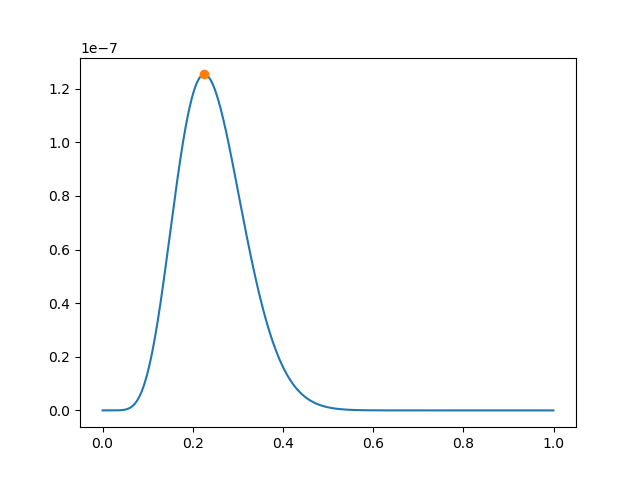
\includegraphics[scale=0.5]{hip1.png}\\
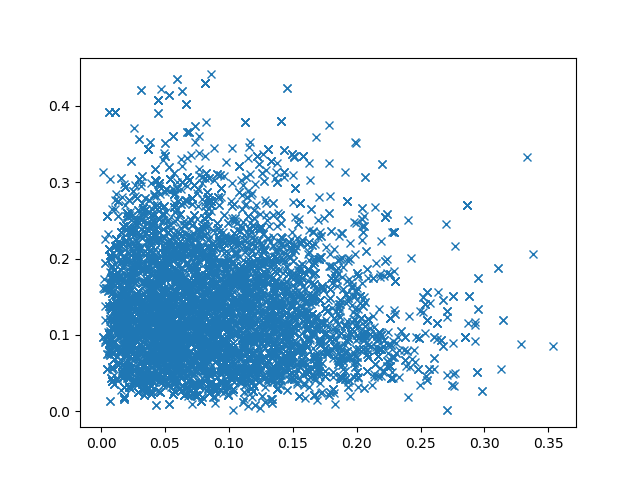
\includegraphics[scale=0.5]{sc1.png}\\
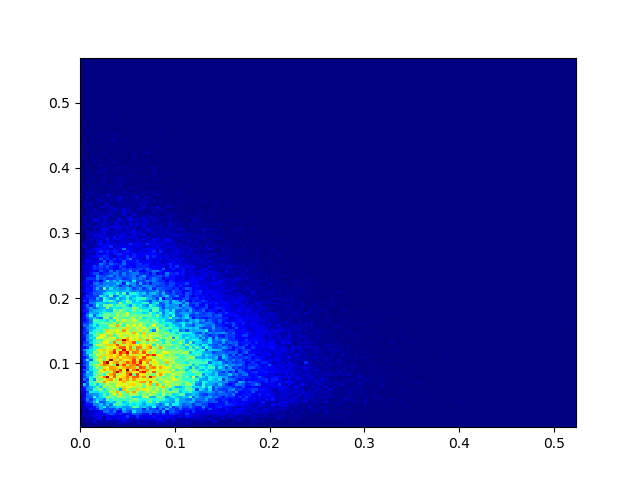
\includegraphics[scale=0.5]{den1.png}\\
\end{center}

\newpage

\begin{center}
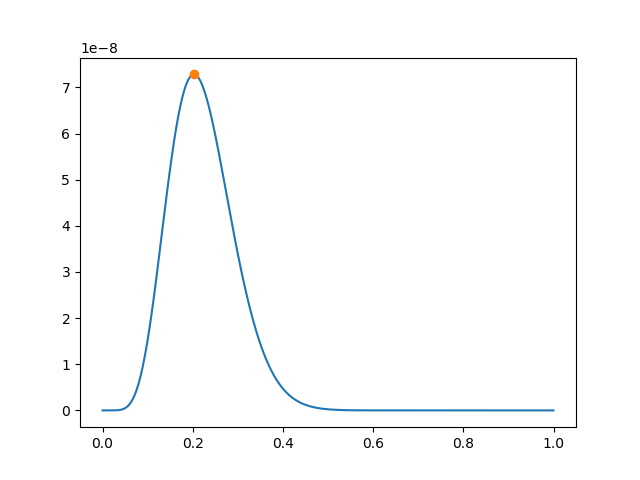
\includegraphics[scale=0.5]{hip2.png}\\
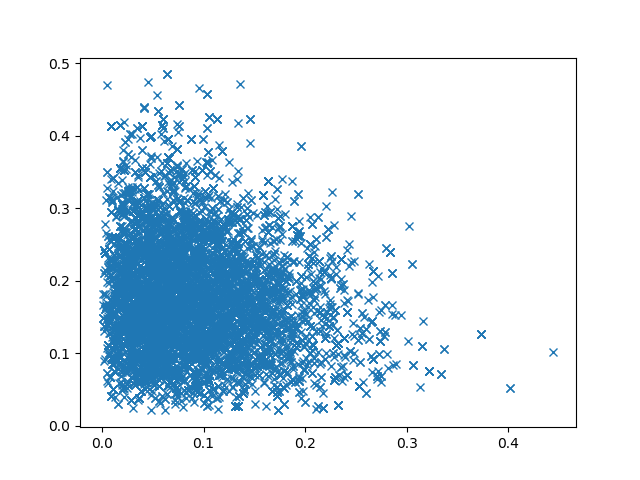
\includegraphics[scale=0.5]{sc2.png}\\
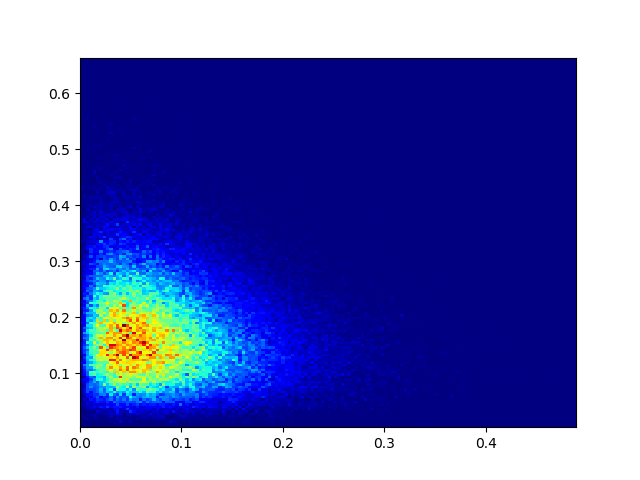
\includegraphics[scale=0.5]{den2.png}\\
\end{center}

\newpage

\begin{center}
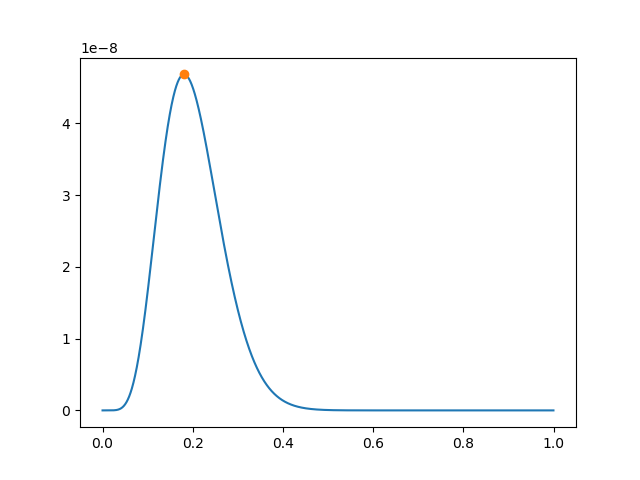
\includegraphics[scale=0.5]{hip3.png}\\
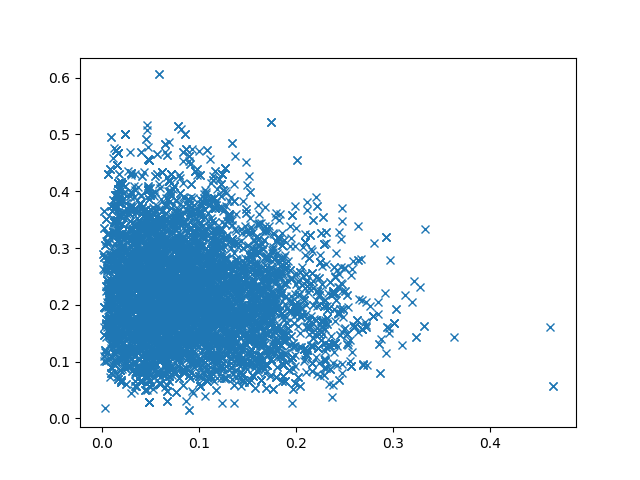
\includegraphics[scale=0.5]{sc3.png}\\
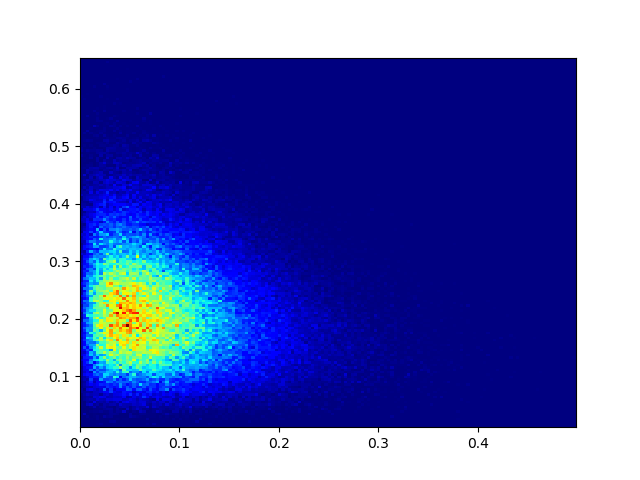
\includegraphics[scale=0.5]{den3.png}\\
\end{center}

\newpage

\begin{center}
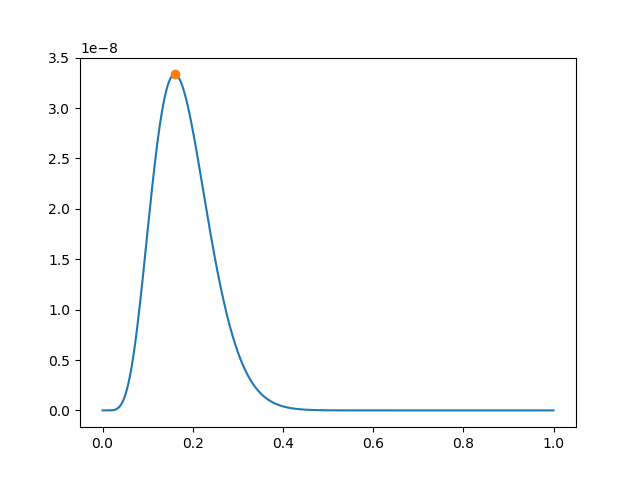
\includegraphics[scale=0.5]{hip4.png}\\
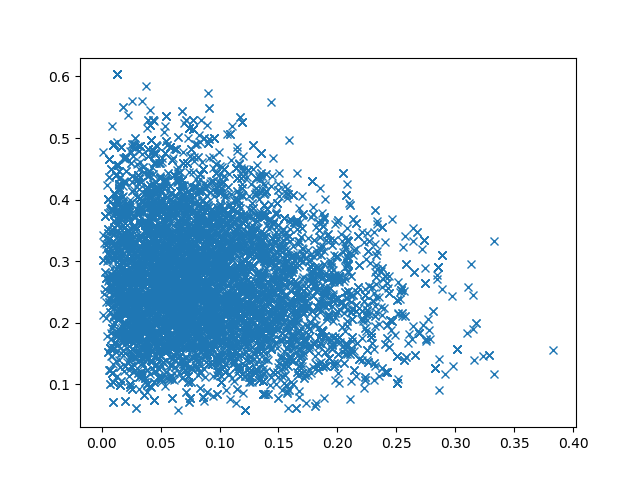
\includegraphics[scale=0.5]{sc4.png}\\
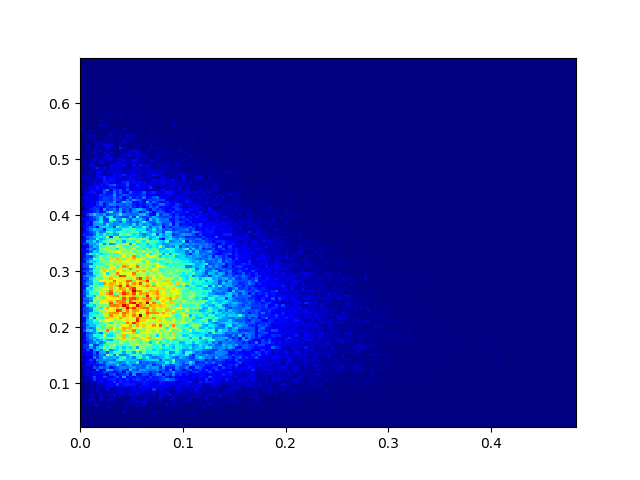
\includegraphics[scale=0.5]{den4.png}\\
\end{center}

\newpage

\begin{center}
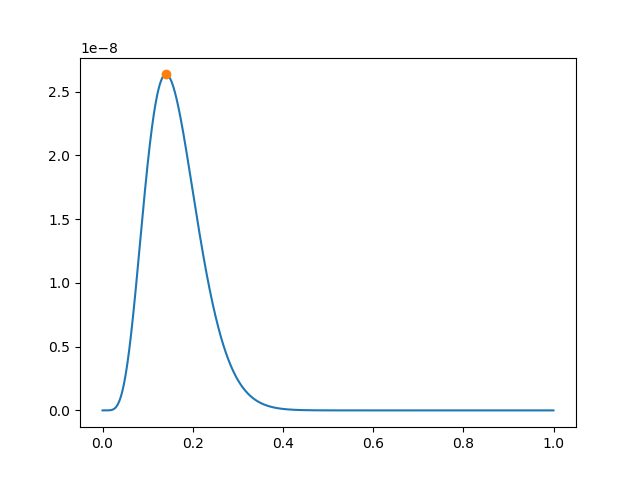
\includegraphics[scale=0.5]{hip5.png}\\
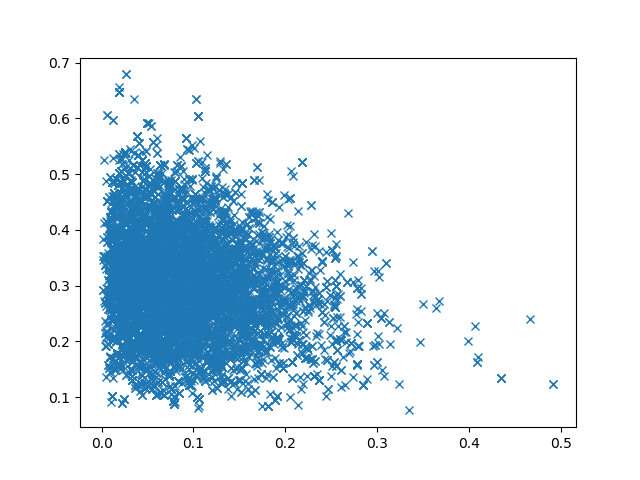
\includegraphics[scale=0.5]{sc5.png}\\
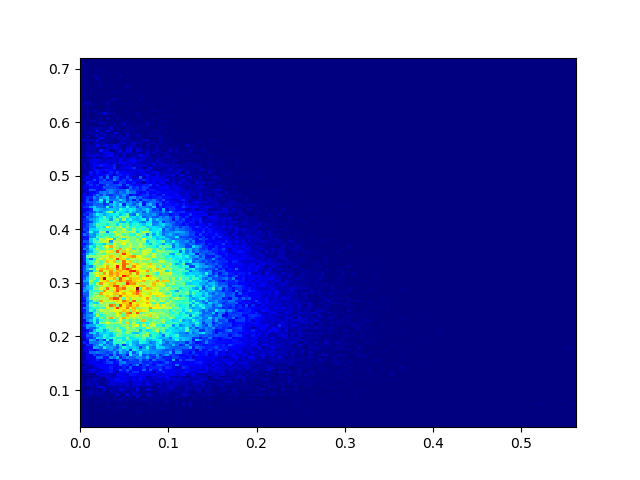
\includegraphics[scale=0.5]{den5.png}\\
\end{center}

\newpage

\begin{center}
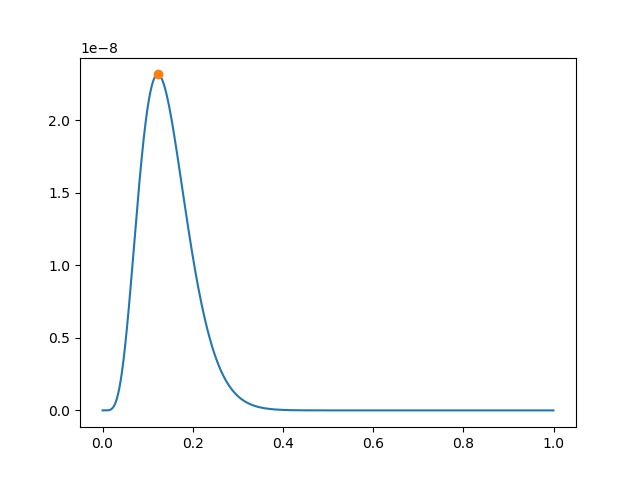
\includegraphics[scale=0.5]{hip6.png}\\
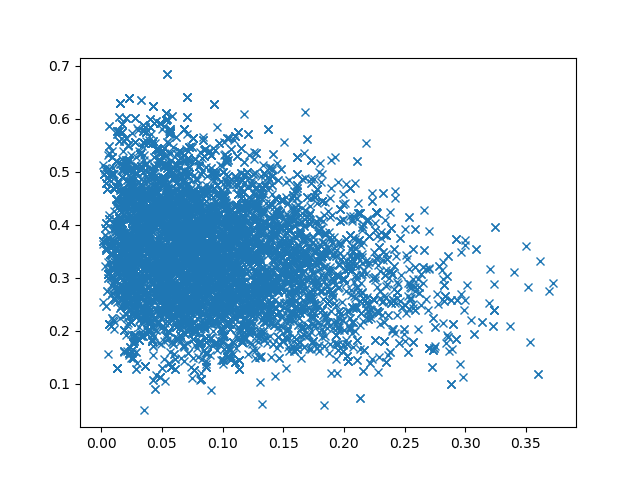
\includegraphics[scale=0.5]{sc6.png}\\
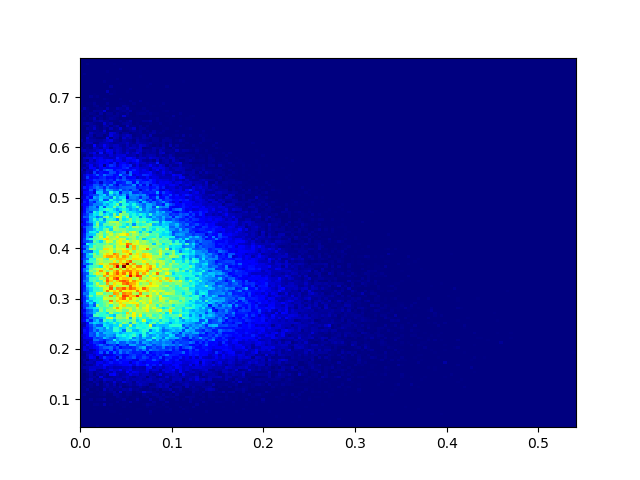
\includegraphics[scale=0.5]{den6.png}\\
\end{center}

\newpage

\begin{center}
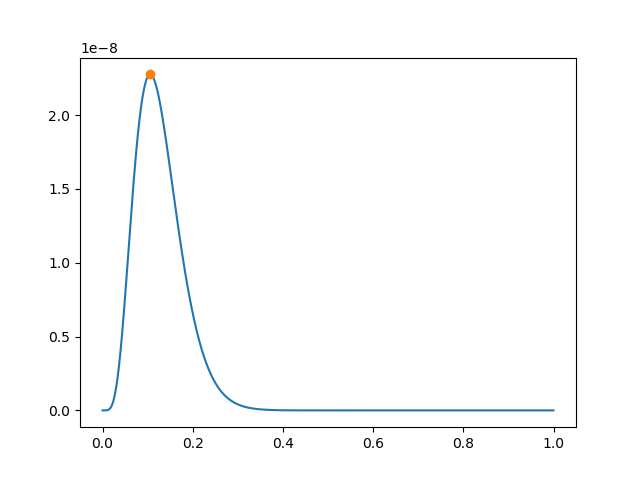
\includegraphics[scale=0.5]{hip7.png}\\
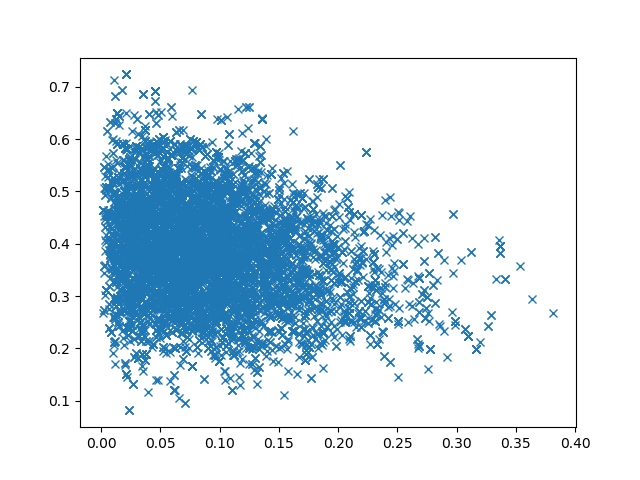
\includegraphics[scale=0.5]{sc7.png}\\
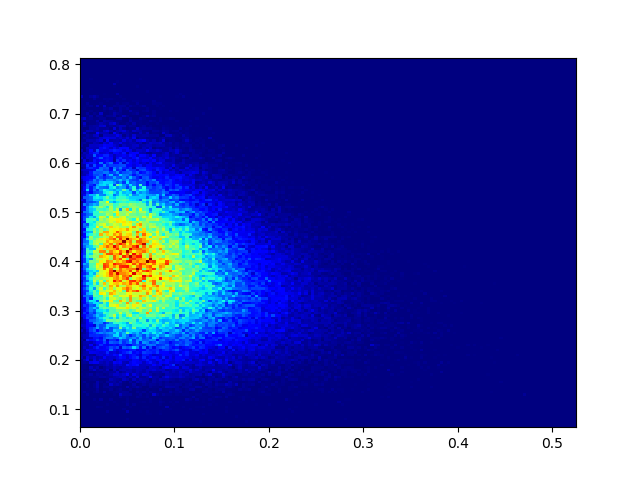
\includegraphics[scale=0.5]{den7.png}\\
\end{center}

\newpage

\begin{center}
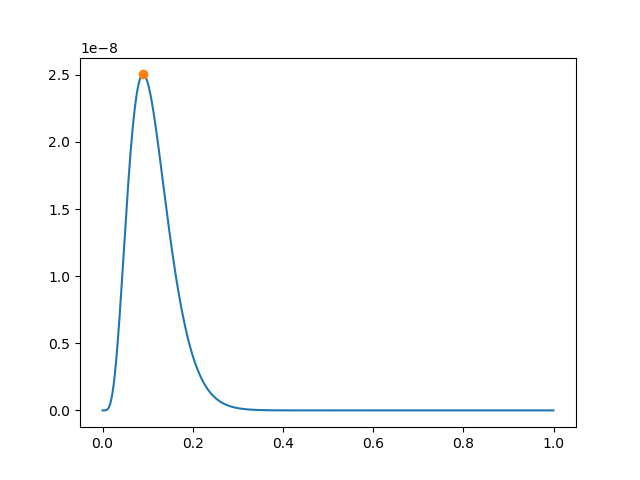
\includegraphics[scale=0.5]{hip8.png}\\
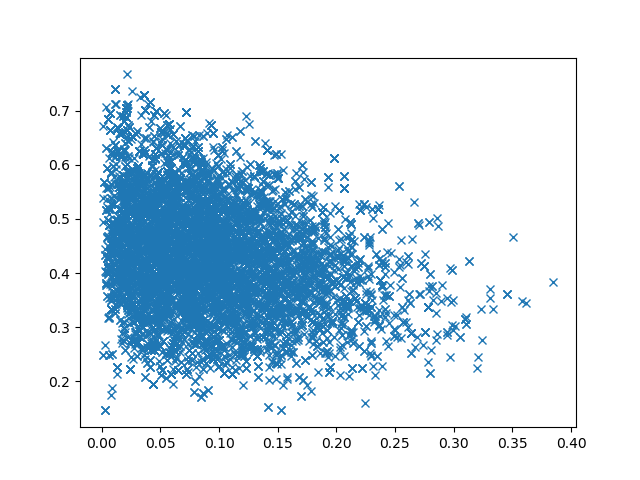
\includegraphics[scale=0.5]{sc8.png}\\
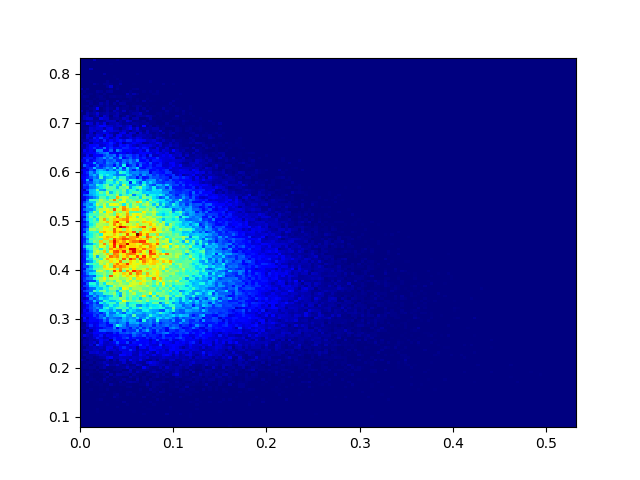
\includegraphics[scale=0.5]{den8.png}\\
\end{center}

\newpage

\begin{center}
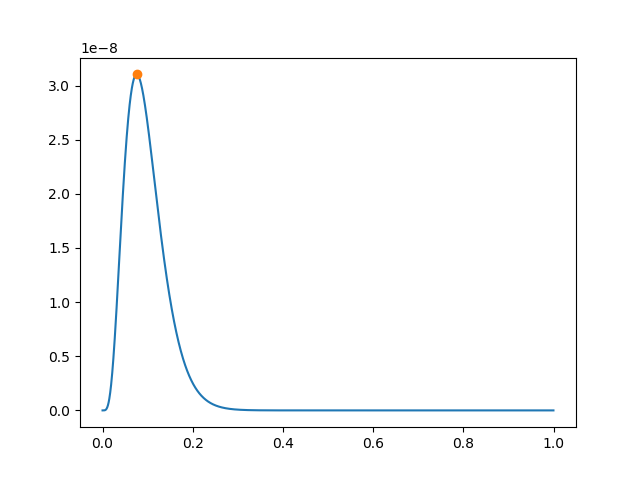
\includegraphics[scale=0.5]{hip9.png}\\
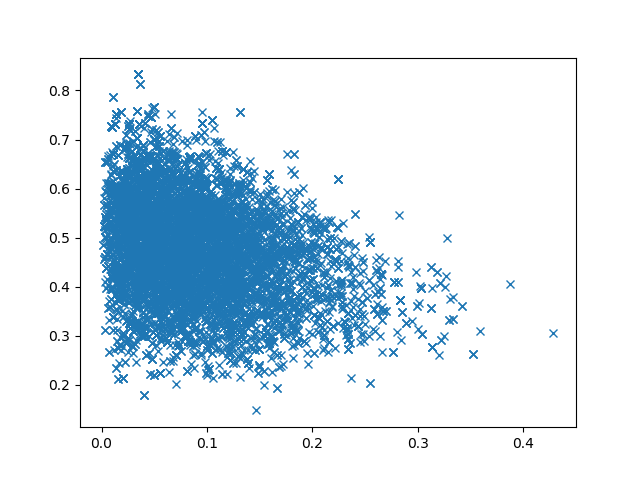
\includegraphics[scale=0.5]{sc9.png}\\
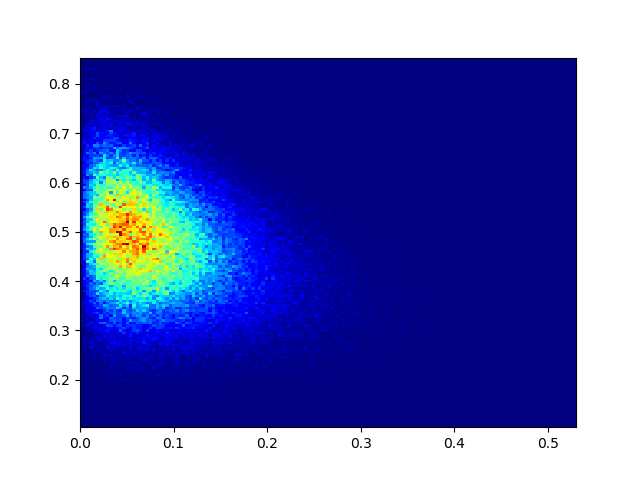
\includegraphics[scale=0.5]{den9.png}\\
\end{center}

\newpage

\begin{center}
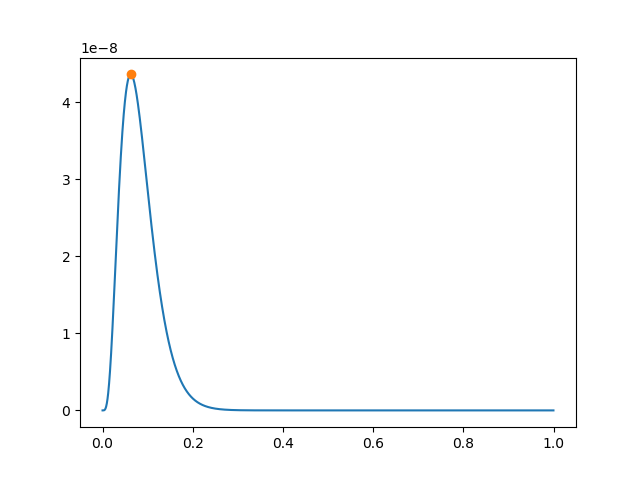
\includegraphics[scale=0.5]{hip10.png}\\
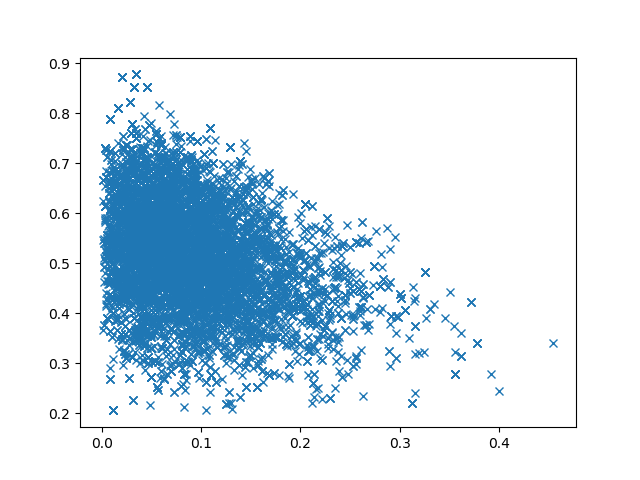
\includegraphics[scale=0.5]{sc10.png}\\
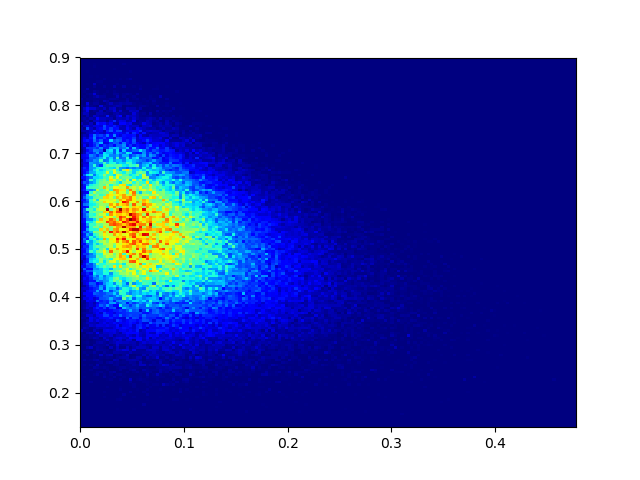
\includegraphics[scale=0.5]{den10.png}\\
\end{center}

\newpage

\begin{center}
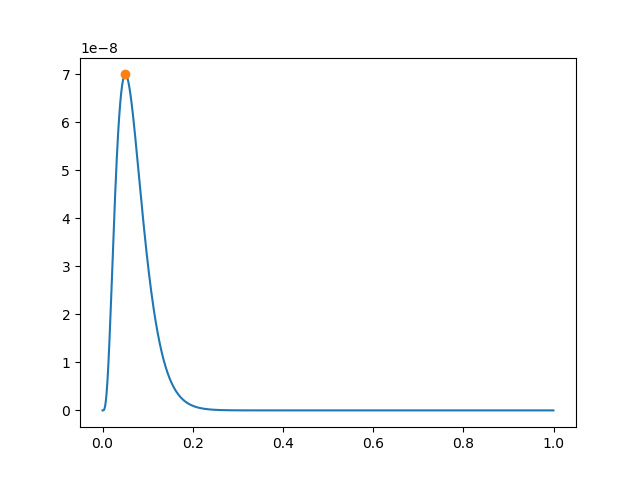
\includegraphics[scale=0.5]{hip11.png}\\
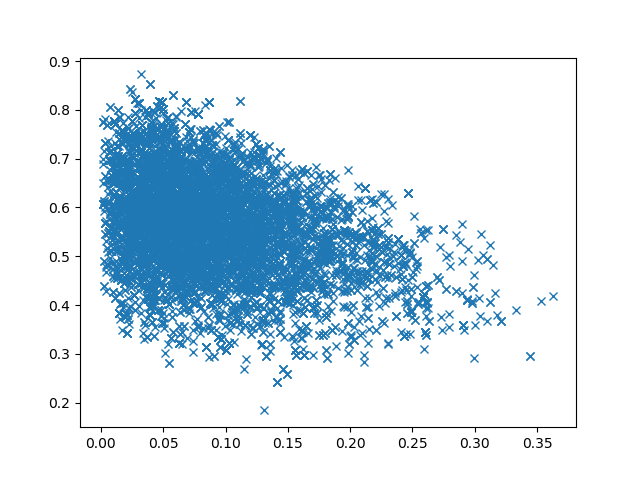
\includegraphics[scale=0.5]{sc11.png}\\
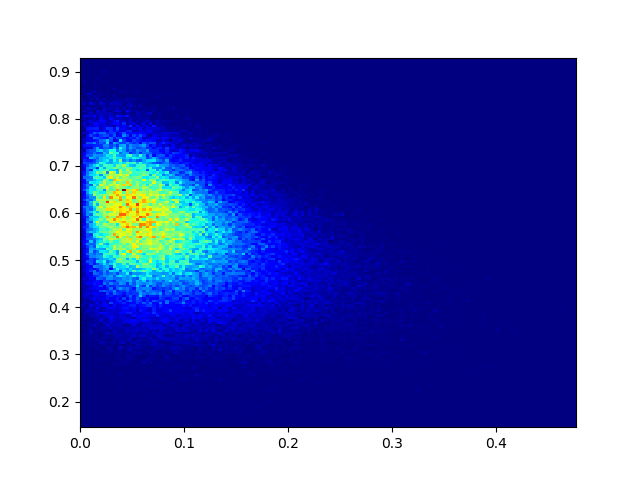
\includegraphics[scale=0.5]{den11.png}\\
\end{center}

\newpage

\begin{center}
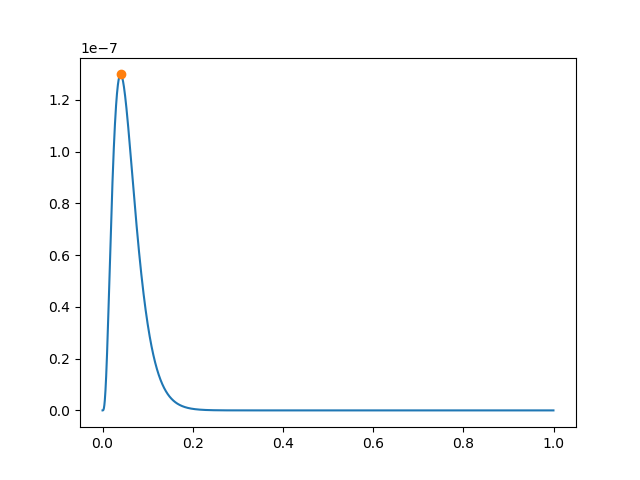
\includegraphics[scale=0.5]{hip12.png}\\
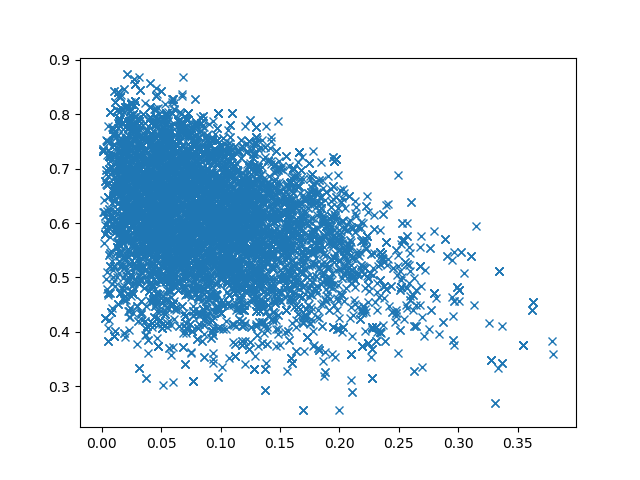
\includegraphics[scale=0.5]{sc12.png}\\
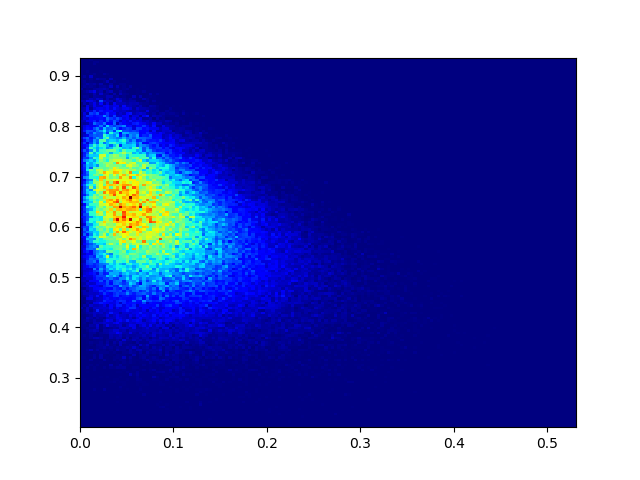
\includegraphics[scale=0.5]{den12.png}\\
\end{center}

\newpage

\begin{center}
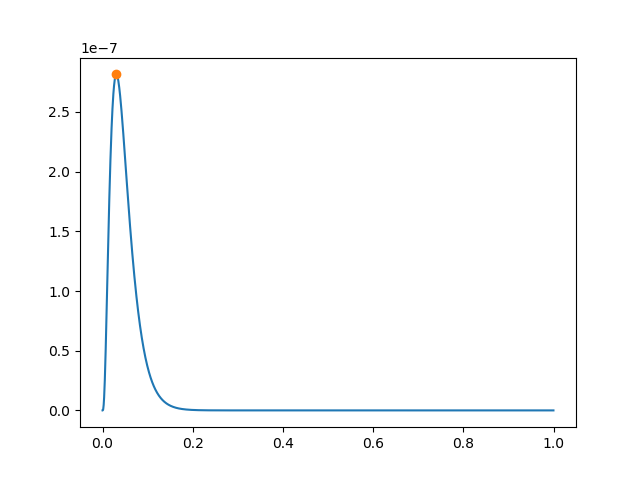
\includegraphics[scale=0.5]{hip13.png}\\
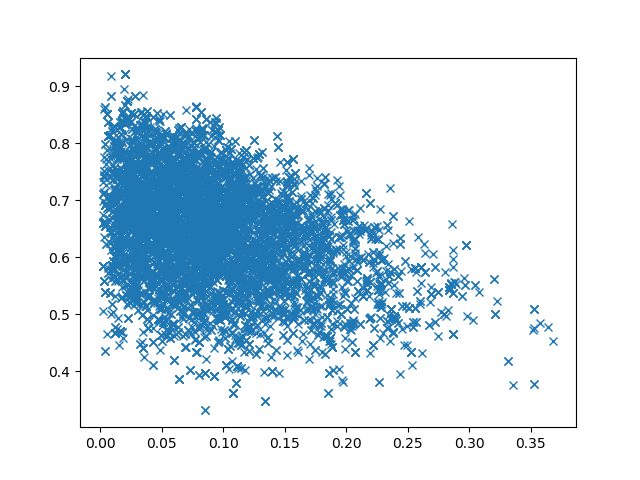
\includegraphics[scale=0.5]{sc13.png}\\
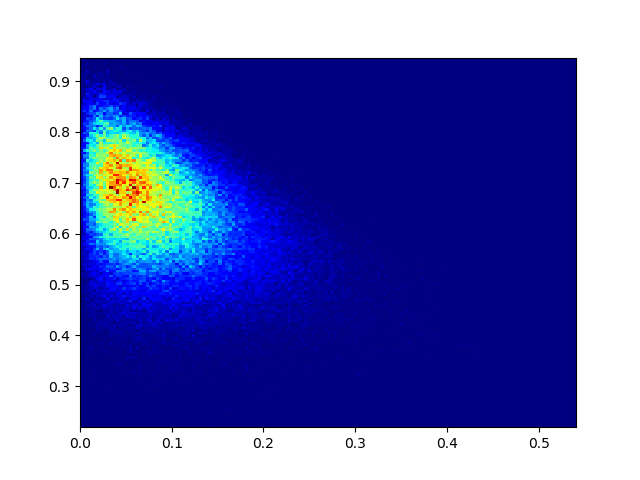
\includegraphics[scale=0.5]{den13.png}\\
\end{center}

\newpage

\begin{center}
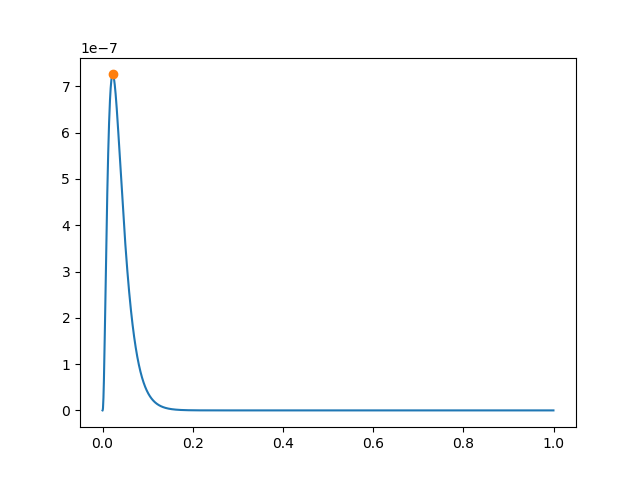
\includegraphics[scale=0.5]{hip14.png}\\
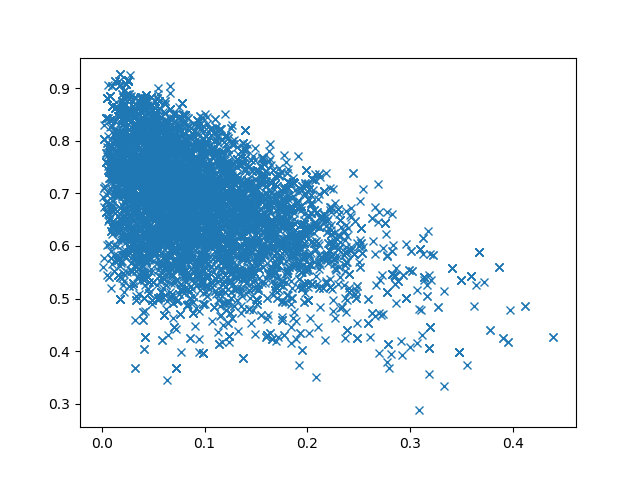
\includegraphics[scale=0.5]{sc14.png}\\
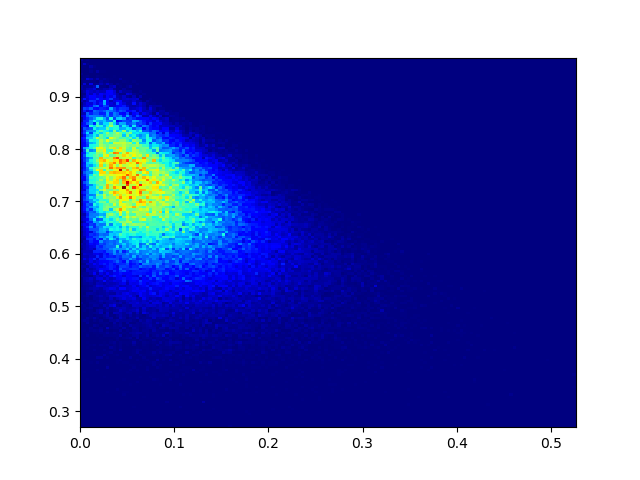
\includegraphics[scale=0.5]{den14.png}\\
\end{center}

\newpage

\begin{center}
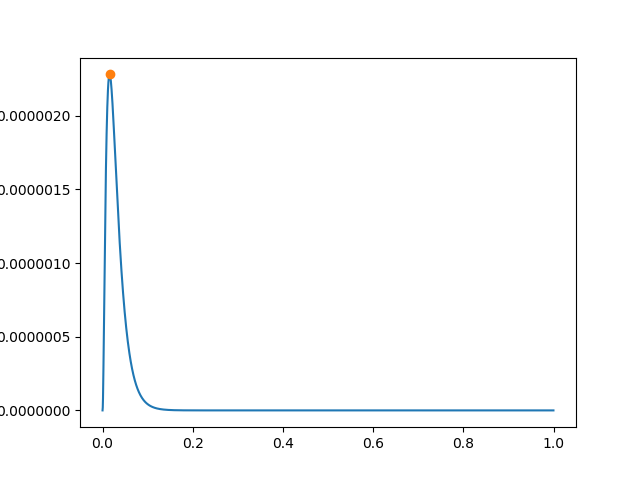
\includegraphics[scale=0.5]{hip15.png}\\
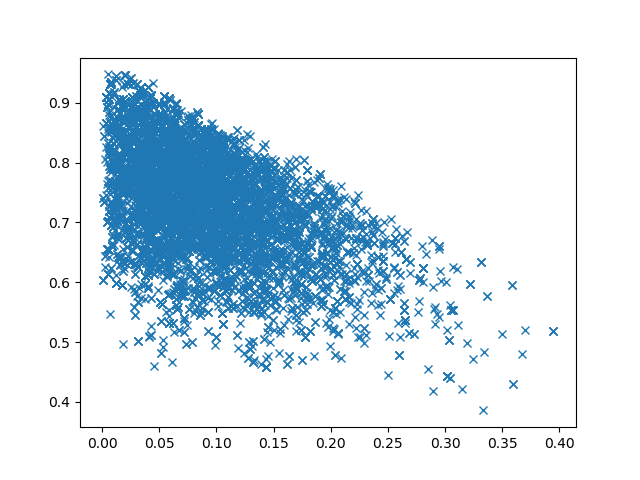
\includegraphics[scale=0.5]{sc15.png}\\
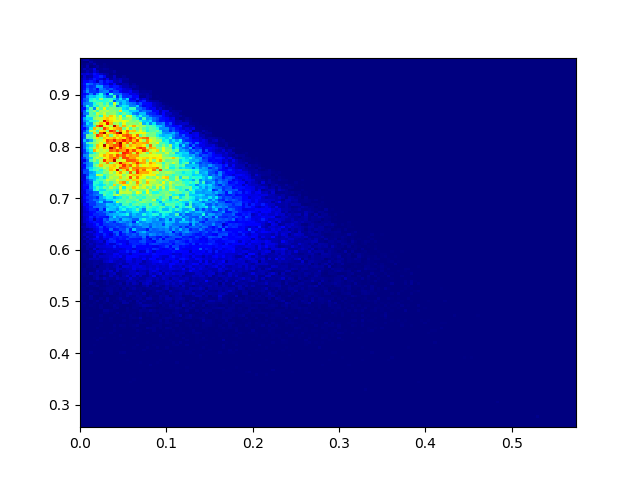
\includegraphics[scale=0.5]{den15.png}\\
\end{center}

\newpage

\begin{center}
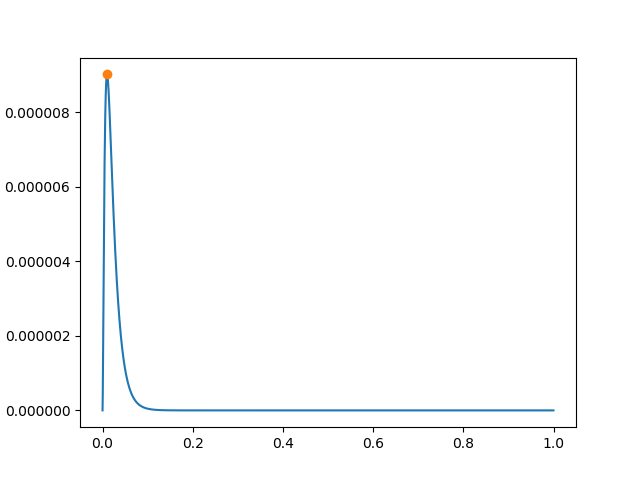
\includegraphics[scale=0.5]{hip16.png}\\
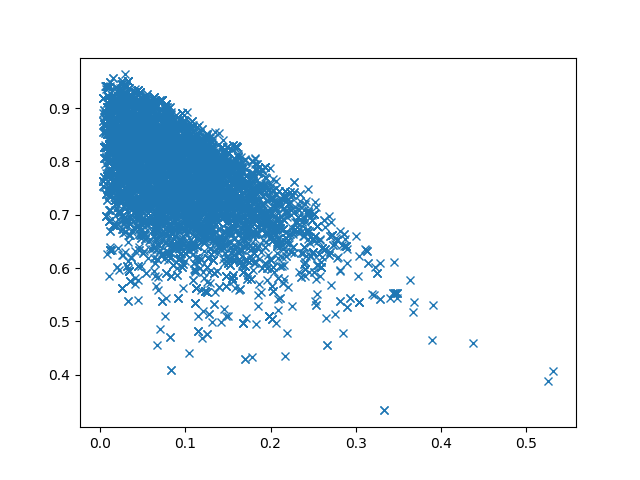
\includegraphics[scale=0.5]{sc16.png}\\
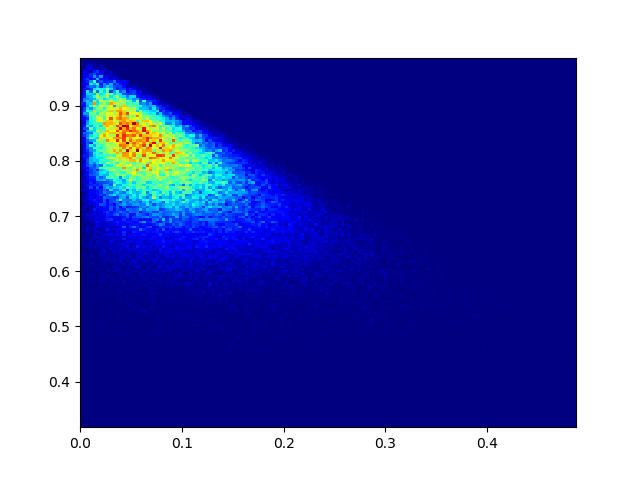
\includegraphics[scale=0.5]{den16.png}\\
\end{center}

\newpage

\begin{center}
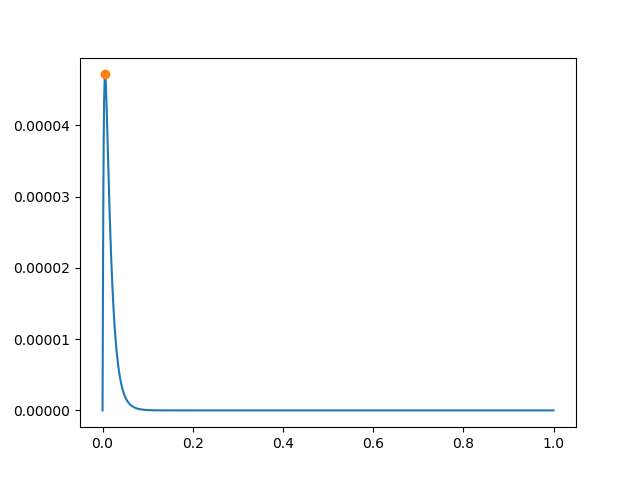
\includegraphics[scale=0.5]{hip17.png}\\
\includegraphics[scale=0.5]{sc17.png}\\
\includegraphics[scale=0.5]{den17.png}\\
\end{center}

\newpage

\begin{center}
\includegraphics[scale=0.5]{hip18.png}\\
\includegraphics[scale=0.5]{sc18.png}\\
\includegraphics[scale=0.5]{den18.png}\\
\end{center}

\newpage

\begin{center}
\includegraphics[scale=0.5]{hip19.png}\\
\includegraphics[scale=0.5]{sc19.png}\\
\includegraphics[scale=0.5]{den19.png}\\
\end{center}

\newpage

\begin{center}
\includegraphics[scale=0.5]{hip20.png}\\
\includegraphics[scale=0.5]{sc20.png}\\
\includegraphics[scale=0.5]{den20.png}\\
\end{center}

\newpage

\begin{center}
\includegraphics[scale=0.5]{hip21.png}\\
\includegraphics[scale=0.5]{sc21.png}\\
\includegraphics[scale=0.5]{den21.png}\\
\end{center}

\newpage

\begin{center}
\includegraphics[scale=0.5]{hip22.png}\\
\includegraphics[scale=0.5]{sc22.png}\\
\includegraphics[scale=0.5]{den22.png}\\
\end{center}

\newpage

\begin{center}
\includegraphics[scale=0.5]{hip23.png}\\
\includegraphics[scale=0.5]{sc23.png}\\
\includegraphics[scale=0.5]{den23.png}\\
\end{center}

\newpage

\begin{center}
\includegraphics[scale=0.5]{hip24.png}\\
\includegraphics[scale=0.5]{sc24.png}\\
\includegraphics[scale=0.5]{den24.png}\\
\end{center}

\newpage

\begin{center}
\includegraphics[scale=0.5]{hip25.png}\\
\includegraphics[scale=0.5]{sc25.png}\\
\includegraphics[scale=0.5]{den25.png}\\
\end{center}

\newpage

\begin{center}
\includegraphics[scale=0.5]{hip26.png}\\
\includegraphics[scale=0.5]{sc26.png}\\
\includegraphics[scale=0.5]{den26.png}\\
\end{center}

\newpage

\begin{center}
\includegraphics[scale=0.5]{hip27.png}\\
\includegraphics[scale=0.5]{sc27.png}\\
\includegraphics[scale=0.5]{den27.png}\\
\end{center}

\newpage

\begin{center}
\includegraphics[scale=0.5]{hip28.png}\\
\includegraphics[scale=0.5]{sc28.png}\\
\includegraphics[scale=0.5]{den28.png}\\
\end{center}

\newpage

\begin{center}
\includegraphics[scale=0.5]{hip29.png}\\
\includegraphics[scale=0.5]{sc29.png}\\
\includegraphics[scale=0.5]{den29.png}\\
\end{center}

\newpage
\begin{center}
\includegraphics[scale=0.5]{hip30.png}\\
\includegraphics[scale=0.5]{sc30.png}\\
\includegraphics[scale=0.5]{den30.png}\\
\end{center}

\newpage

\begin{center}
\includegraphics[scale=0.5]{hip31.png}\\
\includegraphics[scale=0.5]{sc31.png}\\
\includegraphics[scale=0.5]{den31.png}\\
\end{center}

\newpage

\begin{center}
\includegraphics[scale=0.5]{hip32.png}\\
\includegraphics[scale=0.5]{sc32.png}\\
\includegraphics[scale=0.5]{den32.png}\\
\end{center}

\newpage

\begin{center}
\includegraphics[scale=0.5]{hip33.png}\\
\includegraphics[scale=0.5]{sc33.png}\\
\includegraphics[scale=0.5]{den33.png}\\
\end{center}

\newpage

\begin{center}
\includegraphics[scale=0.5]{hip34.png}\\
\includegraphics[scale=0.5]{sc34.png}\\
\includegraphics[scale=0.5]{den34.png}\\
\end{center}

\newpage

\begin{center}
\includegraphics[scale=0.5]{hip35.png}\\
\includegraphics[scale=0.5]{sc35.png}\\
\includegraphics[scale=0.5]{den35.png}\\
\end{center}

\newpage

\begin{center}
\includegraphics[scale=0.5]{hip36.png}\\
\includegraphics[scale=0.5]{sc36.png}\\
\includegraphics[scale=0.5]{den36.png}\\
\end{center}

\subsection{Gráficos de autocorrelação}
\ 

Em seguida alguns gráficos de autocorrelação que evidenciam o que foi mencionado sobre suas propriedades em "$3.2$ Escolha do $\Sigma$":
\newpage

\begin{center}
Gráfico da autocorrelação para $\sigma$s $= 0.1$ e 1000 pontos, para a hipótese na $18_a$ posição:\\
\includegraphics[scale=0.5]{Autocorr1000hip18.png}\\
Gráfico da autocorrelação para $\sigma$s $= 0.1$ e 10000 pontos, para a hipótese na $18_a$ posição:\\
\includegraphics[scale=0.5]{Autocorr10000hip18.png}\\
Gráfico da autocorrelação para $\sigma$s $= 0.5$ e 10000 pontos, para a hipótese na $18_a$ posição:\\
\includegraphics[scale=0.5]{Autocorr10000hip18(0,5).png}\\
\end{center}
\newpage

\begin{center}
Gráfico da autocorrelação para $\sigma$s $= 0.1$ e 1000000 pontos, para a hipótese na $1_a$ posição:\\
\includegraphics[scale=0.5]{Autocorr100000hip1.png}\\
Gráfico da autocorrelação para $\sigma$s $= 0.1$ e 500000 pontos, para a hipótese na $36_a$ posição:\\
\includegraphics[scale=0.5]{Autocorr50000hip36.png}\\

\end{center}








\end{document}























